\documentclass{beamer}
\usepackage[british,spanish]{babel}
\usepackage[utf8]{inputenc}

\usepackage{hyperref}
%\hypersetup{colorlinks=false,linkbordercolor=red,linkcolor=green,pdfborderstyle={/S/U/W 1}}

\usepackage{multirow}

\usepackage{textcomp}

\usepackage{listings}
\lstloadlanguages{Ruby}
\usepackage{cancel}

\usepackage{adjustbox}
\usepackage{lstcustom}

\usepackage{amsmath}

\usepackage{color}
\definecolor{light-gray}{gray}{0.80}
\definecolor{lstbackgroundshellcolor}{named}{light-gray}

\usepackage{tikz}
\newcommand*\circled[1]{\tikz[baseline=(char.base)]{
            \node[shape=circle,draw,inner sep=2pt] (char) {#1};}}

\usepackage[normalem]{ulem}

%\usepackage[acronym,xindy,toc]{glossaries}

\usepackage[acronym,xindy,toc]{glossaries}
\makeglossaries
%\usepackage[xindy]{imakeidx}
%\makeindex


\newcommand{\comment}[2]{#2}aws

\newcommand{\commandinline}[1]{\lstinline[basicstyle=\small\lstfontfamily]{#1}}
\newcommand{\outputcommand}[1]{\color{darkgreen}{#1}}

\graphicspath{ {./images/} }

\title{AWS Identity an Access Management}
%\subtitle[short subtitle]{long subtitle}
\author[C. Cuenca, F. Quintana]{Carmelo Cuenca-Hernández and Francisca Quintana-Domínguez}
%\institute{Escuela Universitaria de Informática}
%\date[04/2013]{Abril - 2013}
\date{}
\titlegraphic{
\includegraphics[width=0.5 \textwidth]{./images/logo_ulpgc_version_horizontal_rgb.eps}}


\pgfdeclareimage[width=2.0\baselineskip]{ulpgc-logo}{images/logosimbolo_secundario_version_vertical}
\setbeamertemplate{footline}{\raisebox{-2ex}{\pgfuseimage{ulpgc-logo}}
  \usebeamerfont{date in head/foot}\insertshortdate{}\hfill
  \usebeamertemplate{navigation symbols}\hfill
  \insertframenumber{}/\inserttotalframenumber}
\setbeamertemplate{sidebar right}{}


\usetheme{Antibes}
%\usetheme{Berlin}

%\usetheme{Warsaw}
%\usecolortheme{albatross}

\selectlanguage{british}



\begin{document}

%
\includegraphics[width= 1.0 \textwidth]{logos3.eps}
\begin{frame}
	\titlepage
\end{frame}


\section*{Outline}
\begin{frame}[fragile, allowframebreaks]
  \frametitle{Outline}
  %\tableofcontents%[part=1,pausesections]
  %\tableofcontents[currentsection,currentsubsection, sectionstyle=show] 
  \tableofcontents[currentsection,sectionstyle=show,hideothersubsections]
\end{frame}

%%%%%%%%%%%%%%%%%%%%%%%%%%%%%%%%%%%%%%%%%%%%%%%%%%%%%%%%%%%%%%%%%%%%%%%%%%%%%%
%\newacronym{<label>}{<abbrv>}{<full>}
%\glsreset{<label>}
%\glsresetall
%\acrlong{<label>}
%\acrfull{<label>}Elastic Load Balancing
%\acrshort{<label>}
%\input{../glossary}

\newacronym{acl}{ACL}{Access Control List}
\newacronym{api}{API}{Application Programming Interface}
\newacronym{aws}{AWS}{Amazon Web Services}
\newacronym{cli}{CLI}{Command Line Interface}
\newacronym{css}{CSS}{cascading style sheets}
\newacronym{ebs}{EBS}{Elastic Block StoAWS Identity an Access Managementrage}
\newacronym{ec2}{EC2}{Amazon Elastic Compute Cloud}
\newacronym{elb}{ELB}{Elastic Load Balancing}
\newacronym{iam}{IAM}{Identity Access Management}
\newacronym{ror}{RoR}{{\href{http://rubyonrails.org/}{Ruby on Rails}}}
\newacronym{rds}{RDS}{Relational Database Service}
\newacronym{rvm}{RVM}{{\href{https://rvm.io/}{Ruby Version Manager}}}
\newacronym{s3}{S3}{Simple Storage Service}
\newacronym{sqs}{SQS}{Amazon Simple Queue Service}
%%%%%%%%%%%%%%%%%%%%%%%%%%%%%%%%%%%%%%%%%%%%%%%%%%%%%%%%%%%%%%%%%%%%%%%%%%%%%%
\section{AWS Identity an Access Management}
\begin{frame}[fragile]
\frametitle{AWS Identity an Access Management}
\acrfull{iam} enables you to control who can do what in your \acrfull{aws} account
\begin{itemize}
 \item Users, Groups, Roles, Permissions
 \item Control
  \begin{itemize}
   \item Centralized
   \item Fine-grained (APIs, resources and \acrshort{aws} Management Console)
  \end{itemize}

 \item Security
 \begin{itemize}
    \item Secure by default
    \item Multiple users, individual security credentials and permissions
  \end{itemize}
\end{itemize}
\end{frame}
%%%%%%%%%%%%%%%%%%%%%%%%%%%%%%%%%%%%%%%%%%%%%%%%%%%%%%%%%%%%%%%%%%%%%%%%%%%%%
%%%%%%%%%%%%%%%%%%%%%%%%%%%%%%%%%%%%%%%%%%%%%%%%%%%%%%%%%%%%%%%%%%%%%%%%%%%%%%
\section{Top 10 IAM best practices}
\begin{frame}[fragile]
\frametitle{Top 10 IAM best practices}
\begin{columns}
\column{0.35 \textwidth}
\begin{itemize}
 \item Users
 \item Groups
 \item Permissions
 \item Passwords
 \item MFA
 \item Sharing
 \item Rotation
 \item Conditions
 \item Root
\end{itemize}
\column{0.65 \textwidth}
 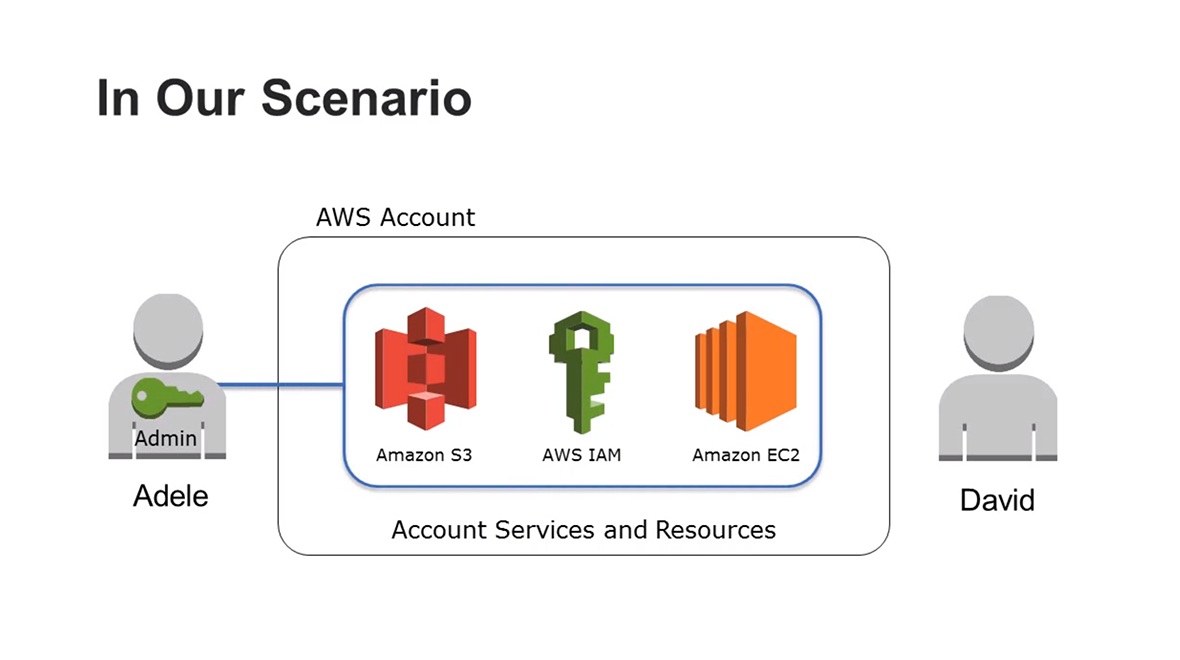
\includegraphics[width= 1.0 \textwidth]{scenario.png}
\end{columns}
\end{frame}
%%%%%%%%%%%%%%%%%%%%%%%%%%%%%%%%%%%%%%%%%%%%%%%%%%%%%%%%%%%%%%%%%%%%%%%%%%%%%
%%%%%%%%%%%%%%%%%%%%%%%%%%%%%%%%%%%%%%%%%%%%%%%%%%%%%%%%%%%%%%%%%%%%%%%%%%%%%%
\section{Create individual users}
\begin{frame}[fragile]
\frametitle{Create individual users}
How to steps
\begin{itemize}
 \item Identify which \acrshort{iam} you want to create
 \item Use the \acrshort{iam} Console, \acrfull{cli} or \acrfull{api} to:
  \begin{itemize}
 \item Create user
 \item Assign credentials
 \item Assign Permissions
\end{itemize}
\end{itemize}
\end{frame}
%%%%%%%%%%%%%%%%%%%%%%%%%%%%%%%%%%%%%%%%%%%%%%%%%%%%%%%%%%%%%%%%%%%%%%%%%%%%%
%%%%%%%%%%%%%%%%%%%%%%%%%%%%%%%%%%%%%%%%%%%%%%%%%%%%%%%%%%%%%%%%%%%%%%%%%%%%%%
\section{Users}
\begin{frame}[fragile]
\frametitle{Users}
\begin{itemize}
\item Create a new user
\begin{itemize}
 \item Navigate to the Secure \acrshort{aws} Access Control Dashboard 
 \item Create a New User with \texttt{Name: `admin'} in the Secure \acrshort{aws} Access Control Dashboard
 \item Download and save in a secure place the Security Credentials (They will be needed)
 \begin{center}
 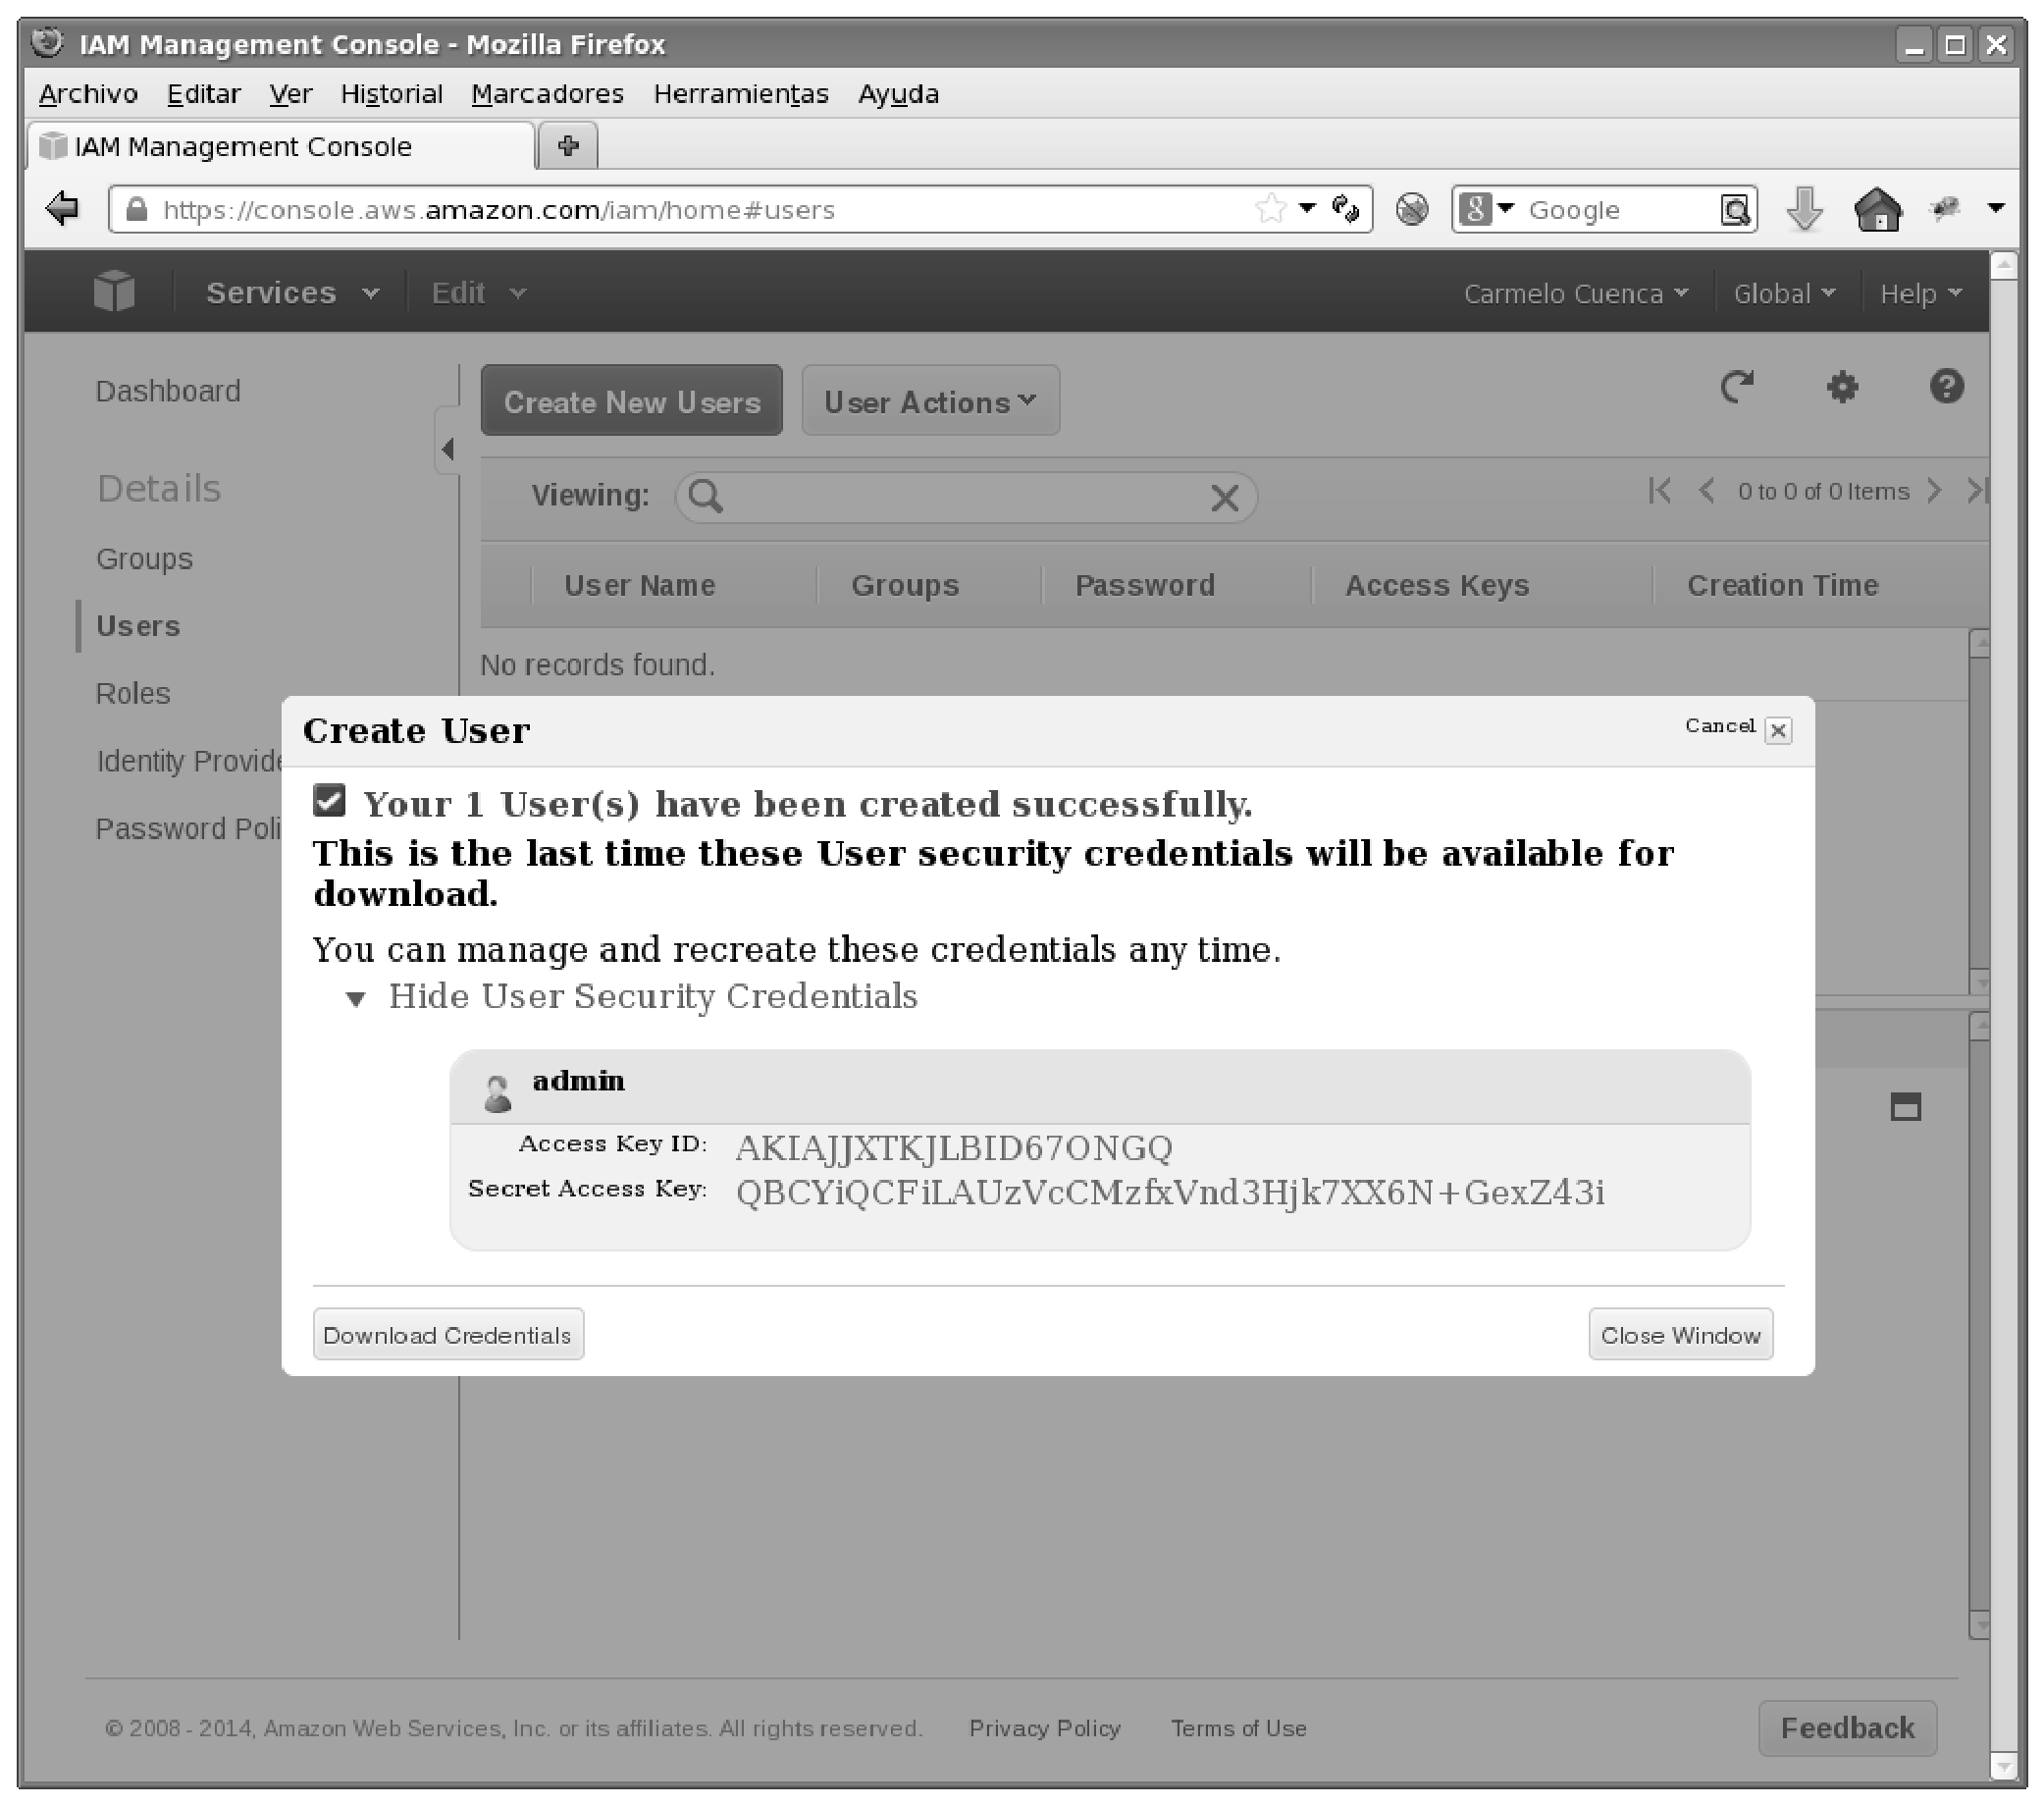
\includegraphics[scale=0.10]{credentials.eps}
 \end{center}
\end{itemize}
\end{itemize}
\end{frame}
%%%%%%%%%%%%%%%%%%%%%%%%%%%%%%%%%%%%%%%%%%%%%%%%%%%%%%%%%%%%%%%%%%%%%%%%%%%%%
%%%%%%%%%%%%%%%%%%%%%%%%%%%%%%%%%%%%%%%%%%%%%%%%%%%%%%%%%%%%%%%%%%%%%%%%%%%%%%
\section{Groups and Permissions}
\begin{frame}[fragile]
\frametitle{Groups}
\begin{itemize}
\item Benefits
\begin{itemize}
 \item Easier to assign the same permissions to multiple users
 \item Simpler to re-assign permissions based on change in responsabilies
 \item Only one change to update permissions to multiple users
\end{itemize}
\item How to steps
\begin{itemize}
\item Map permissions to a specific business function
\item Assign users to that function
\item Manage groups in the Group section of the \acrshort{iam} Console
\end{itemize}
\item Create a New Group with \texttt{Name: ``Administrators''} and assign ``Administrator Access'' in order to provides full access to \acrshort{aws} services and resources
\end{itemize}
\end{frame}
%%%%%%%%%%%%%%%%%%%%%%%%%%%%%%%%%%%%%%%%%%%%%%%%%%%%%%%%%%%%%%%%%%%%%%%%%%%%%
\begin{frame}[fragile]
\frametitle{User Management}
\begin{itemize}
\item Add user \texttt{``admin''} to Group \texttt{``Administrator''}
\begin{center}
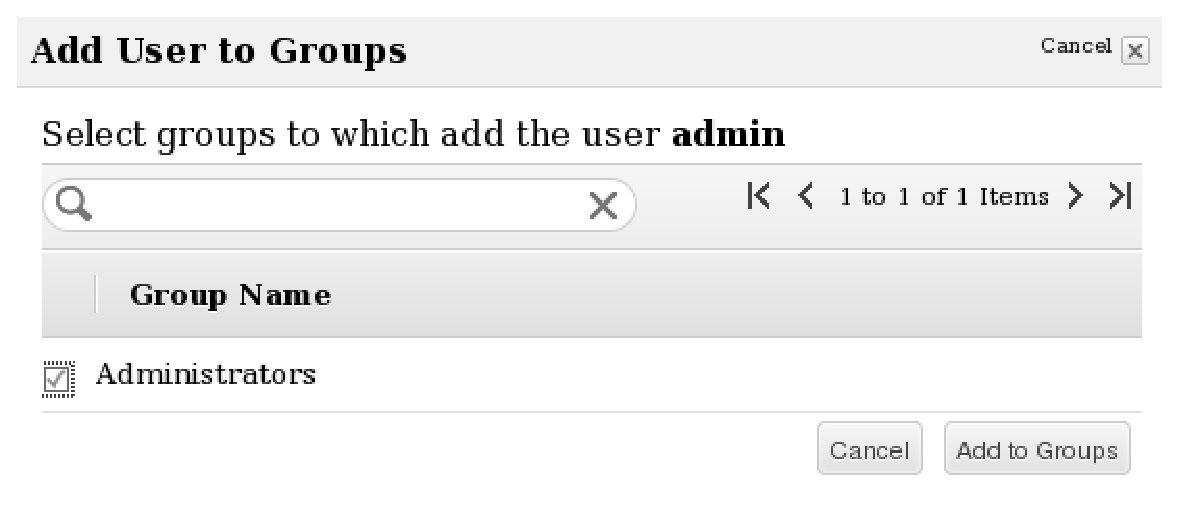
\includegraphics[scale=0.15]{addusertogroup.eps}
\end{center}
\item Assign a password to user \texttt{``admin''} in ``Security Credentials''Users tab
\begin{center}
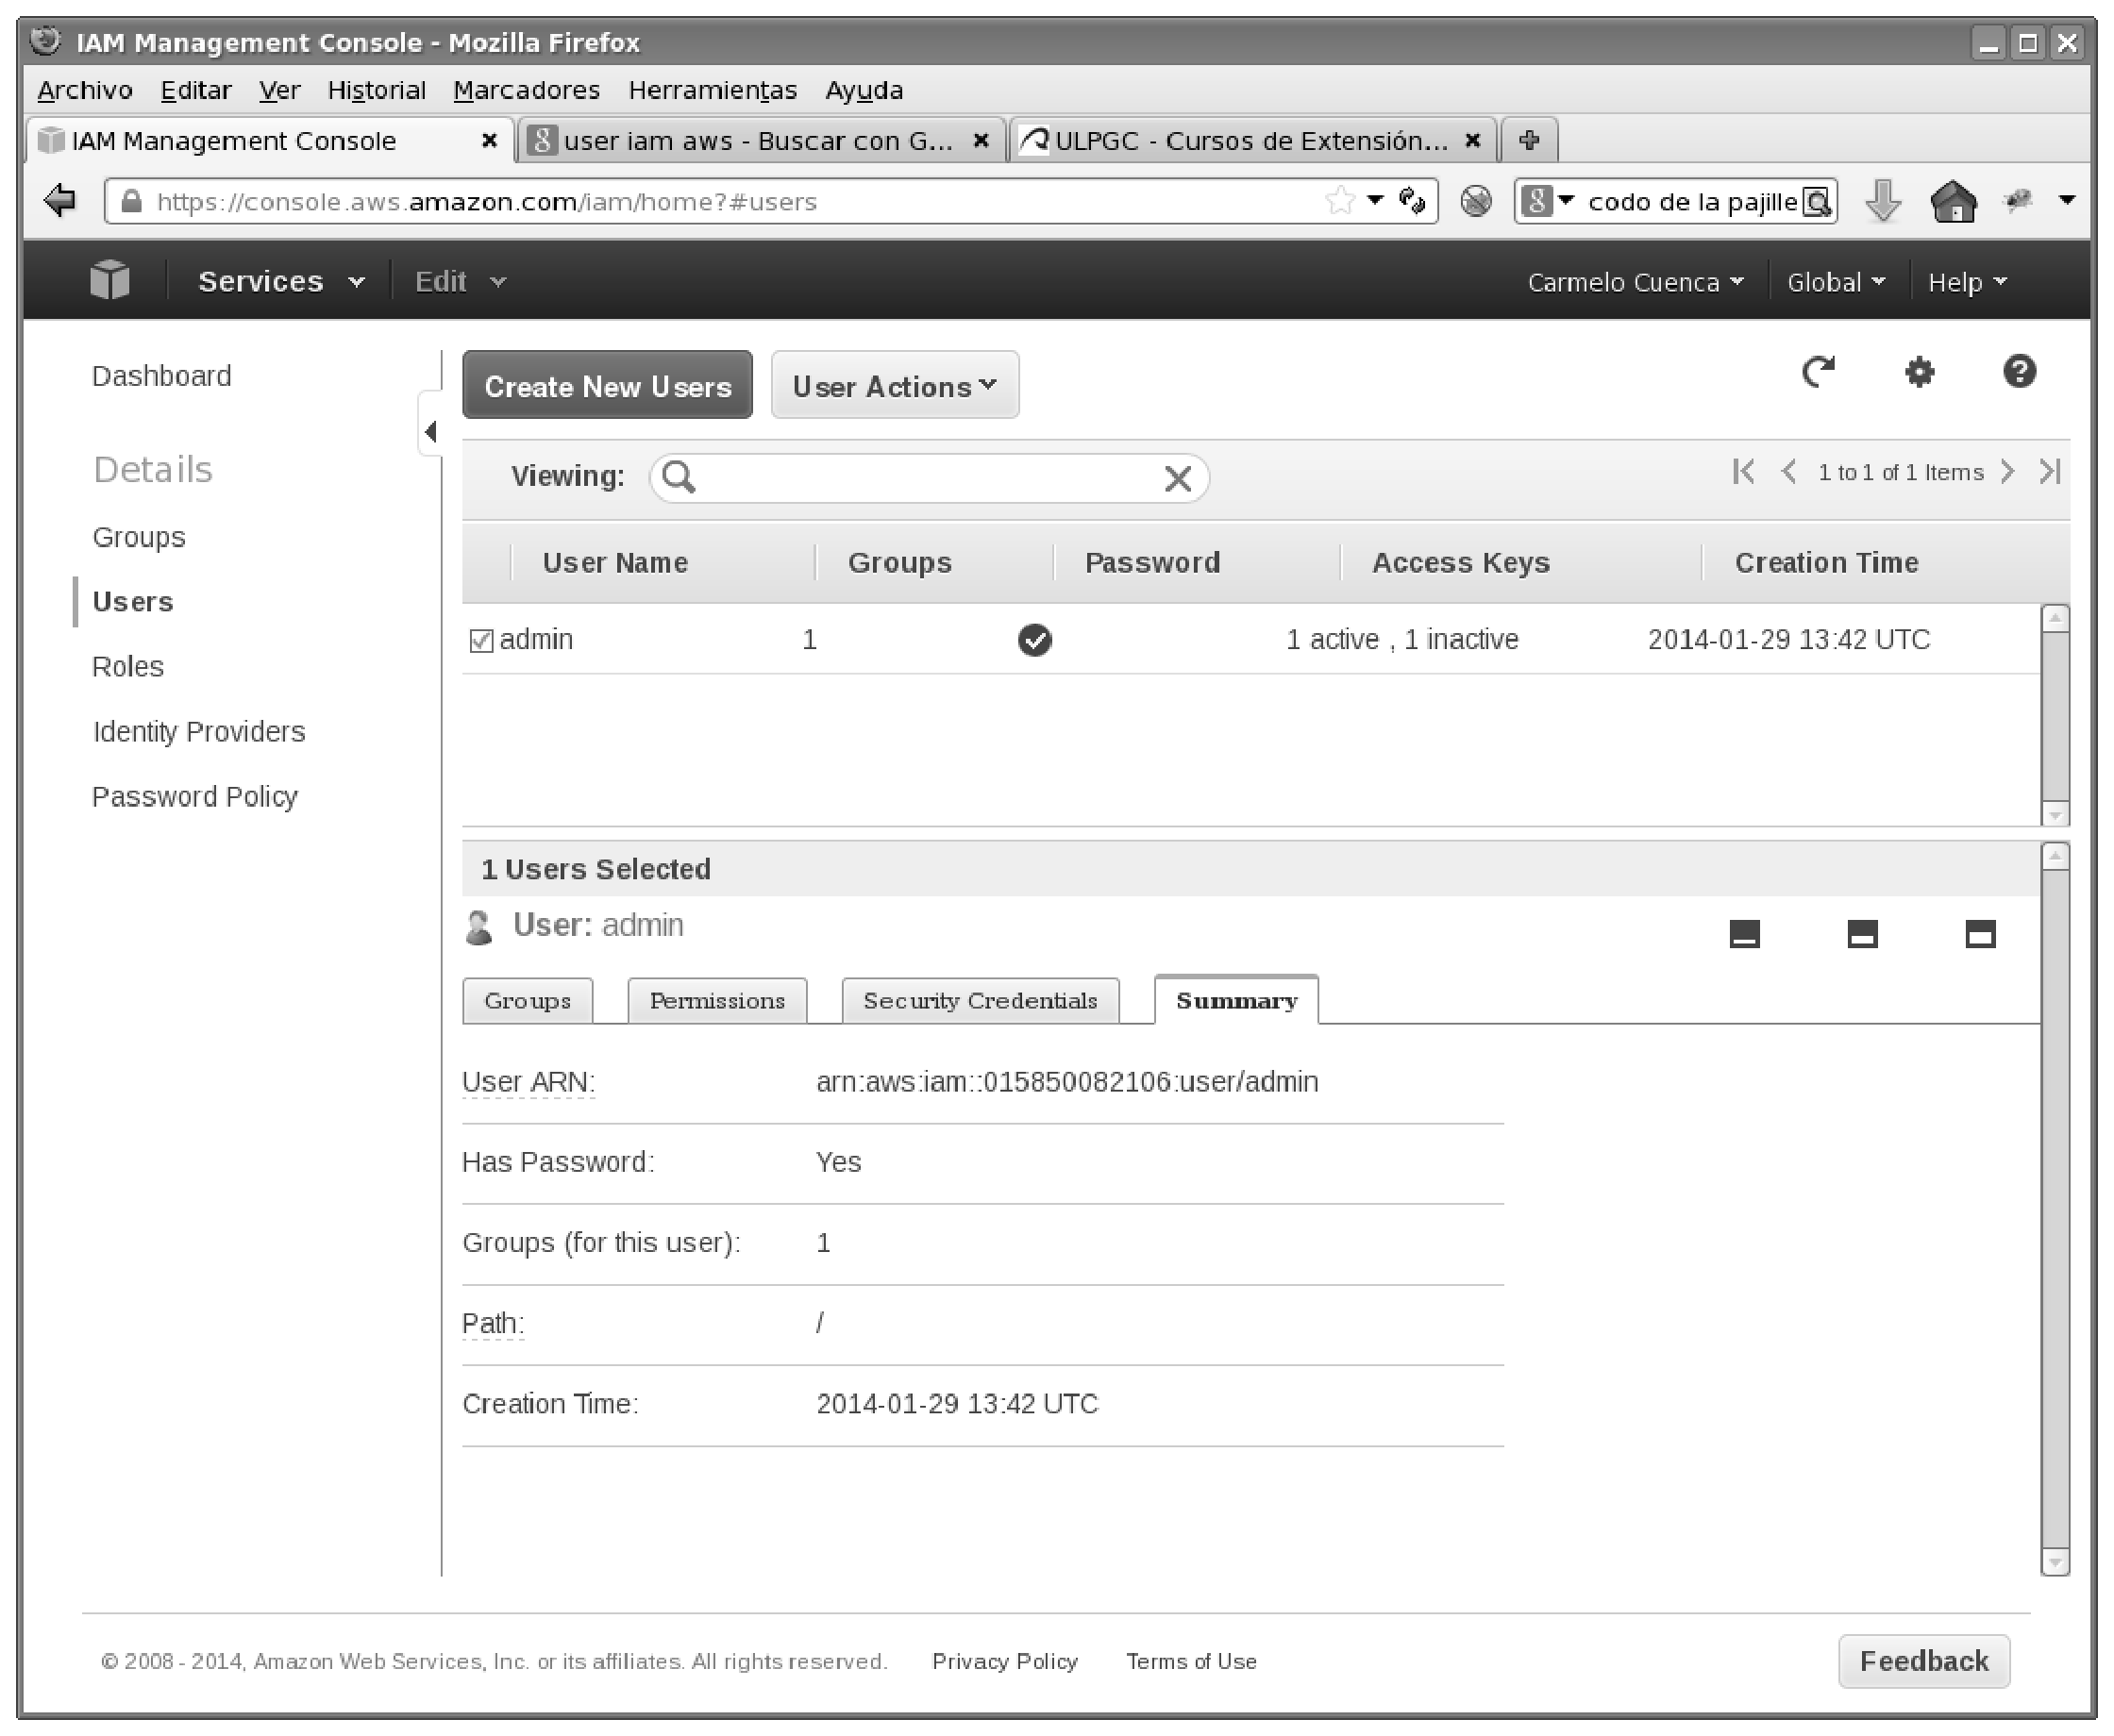
\includegraphics[scale=0.10]{summary.eps}
\end{center}
\end{itemize}
\end{frame}
%%%%%%%%%%%%%%%%%%%%%%%%%%%%%%%%%%%%%%%%%%%%%%%%%%%%%%%%%%%%%%%%%%%%%%%%%%%%%
%%%%%%%%%%%%%%%%%%%%%%%%%%%%%%%%%%%%%%%%%%%%%%%%%%%%%%%%%%%%%%%%%%%%%%%%%%%%%
\begin{frame}[fragile]
\frametitle{IAM User Sign-In URL}
\begin{itemize}
\item Navigate to IAM User Sign-In URL  \url{https://perdidita.signin.aws.amazon.com/console}
\item Signin as user \texttt{``admin''}
\begin{columns}
\column{0.65 \textwidth}
\begin{center}
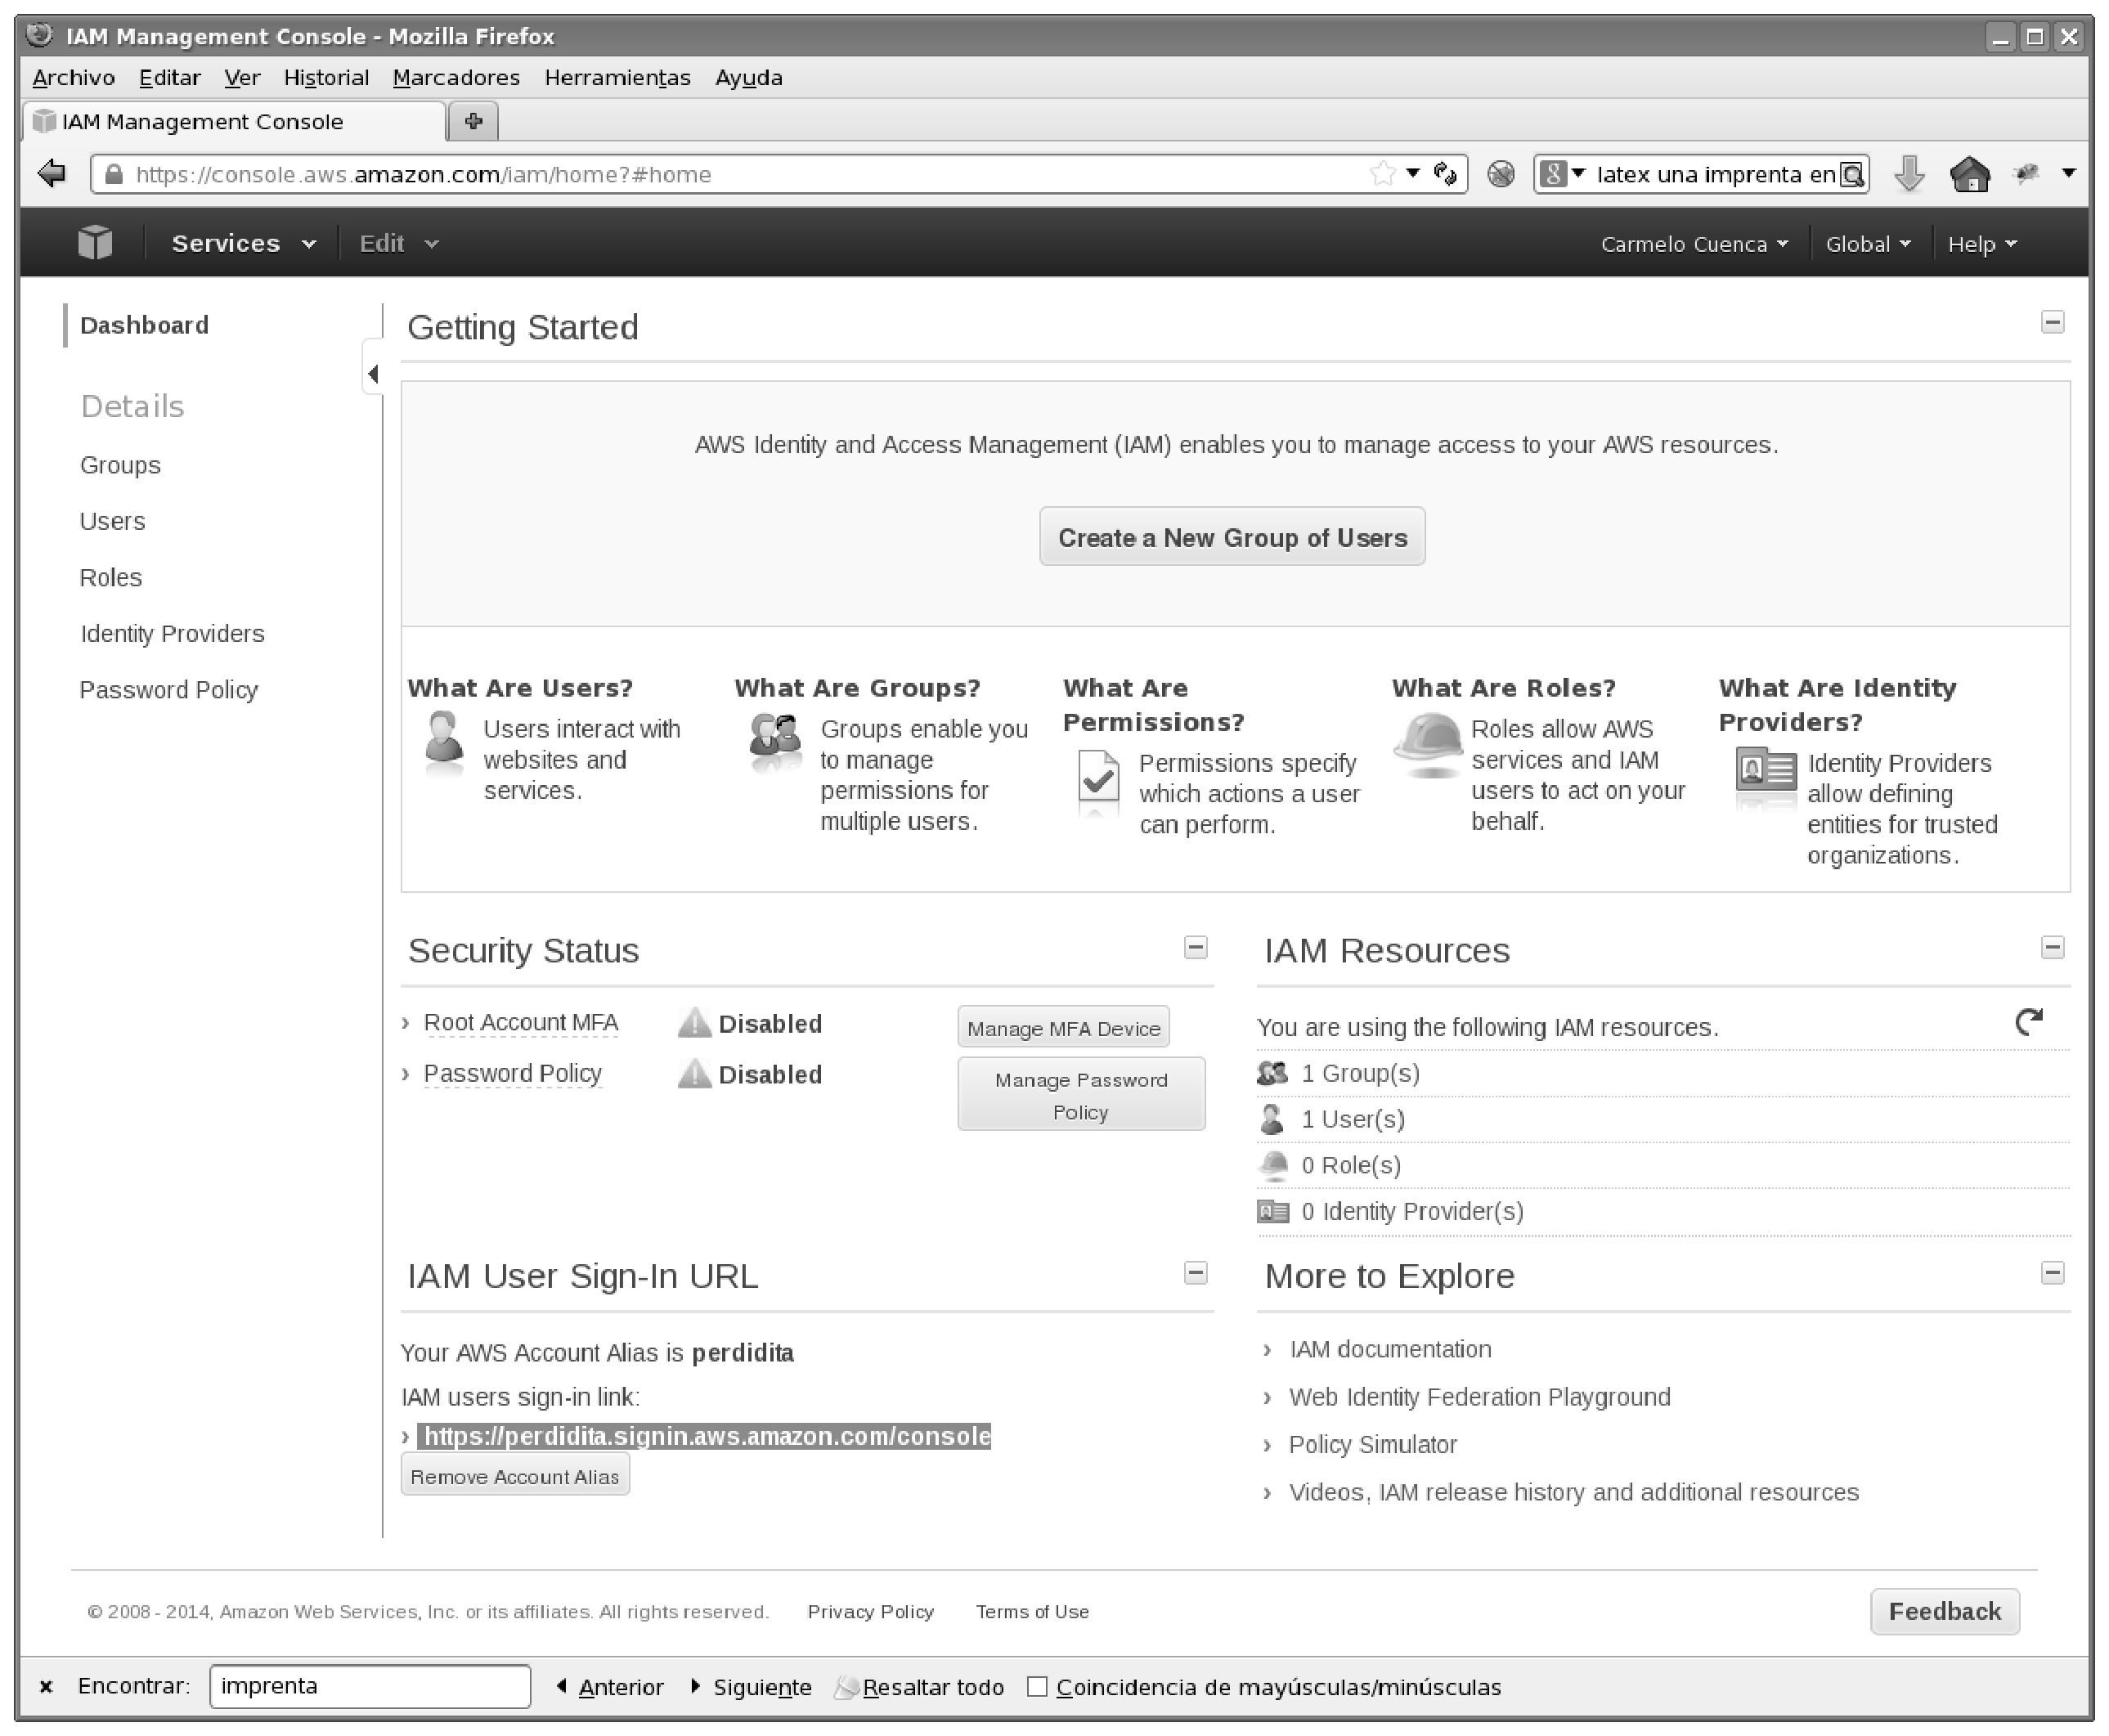
\includegraphics[scale=0.10]{siginurl.eps}
\end{center}
\column{0.35 \textwidth}
\begin{center}
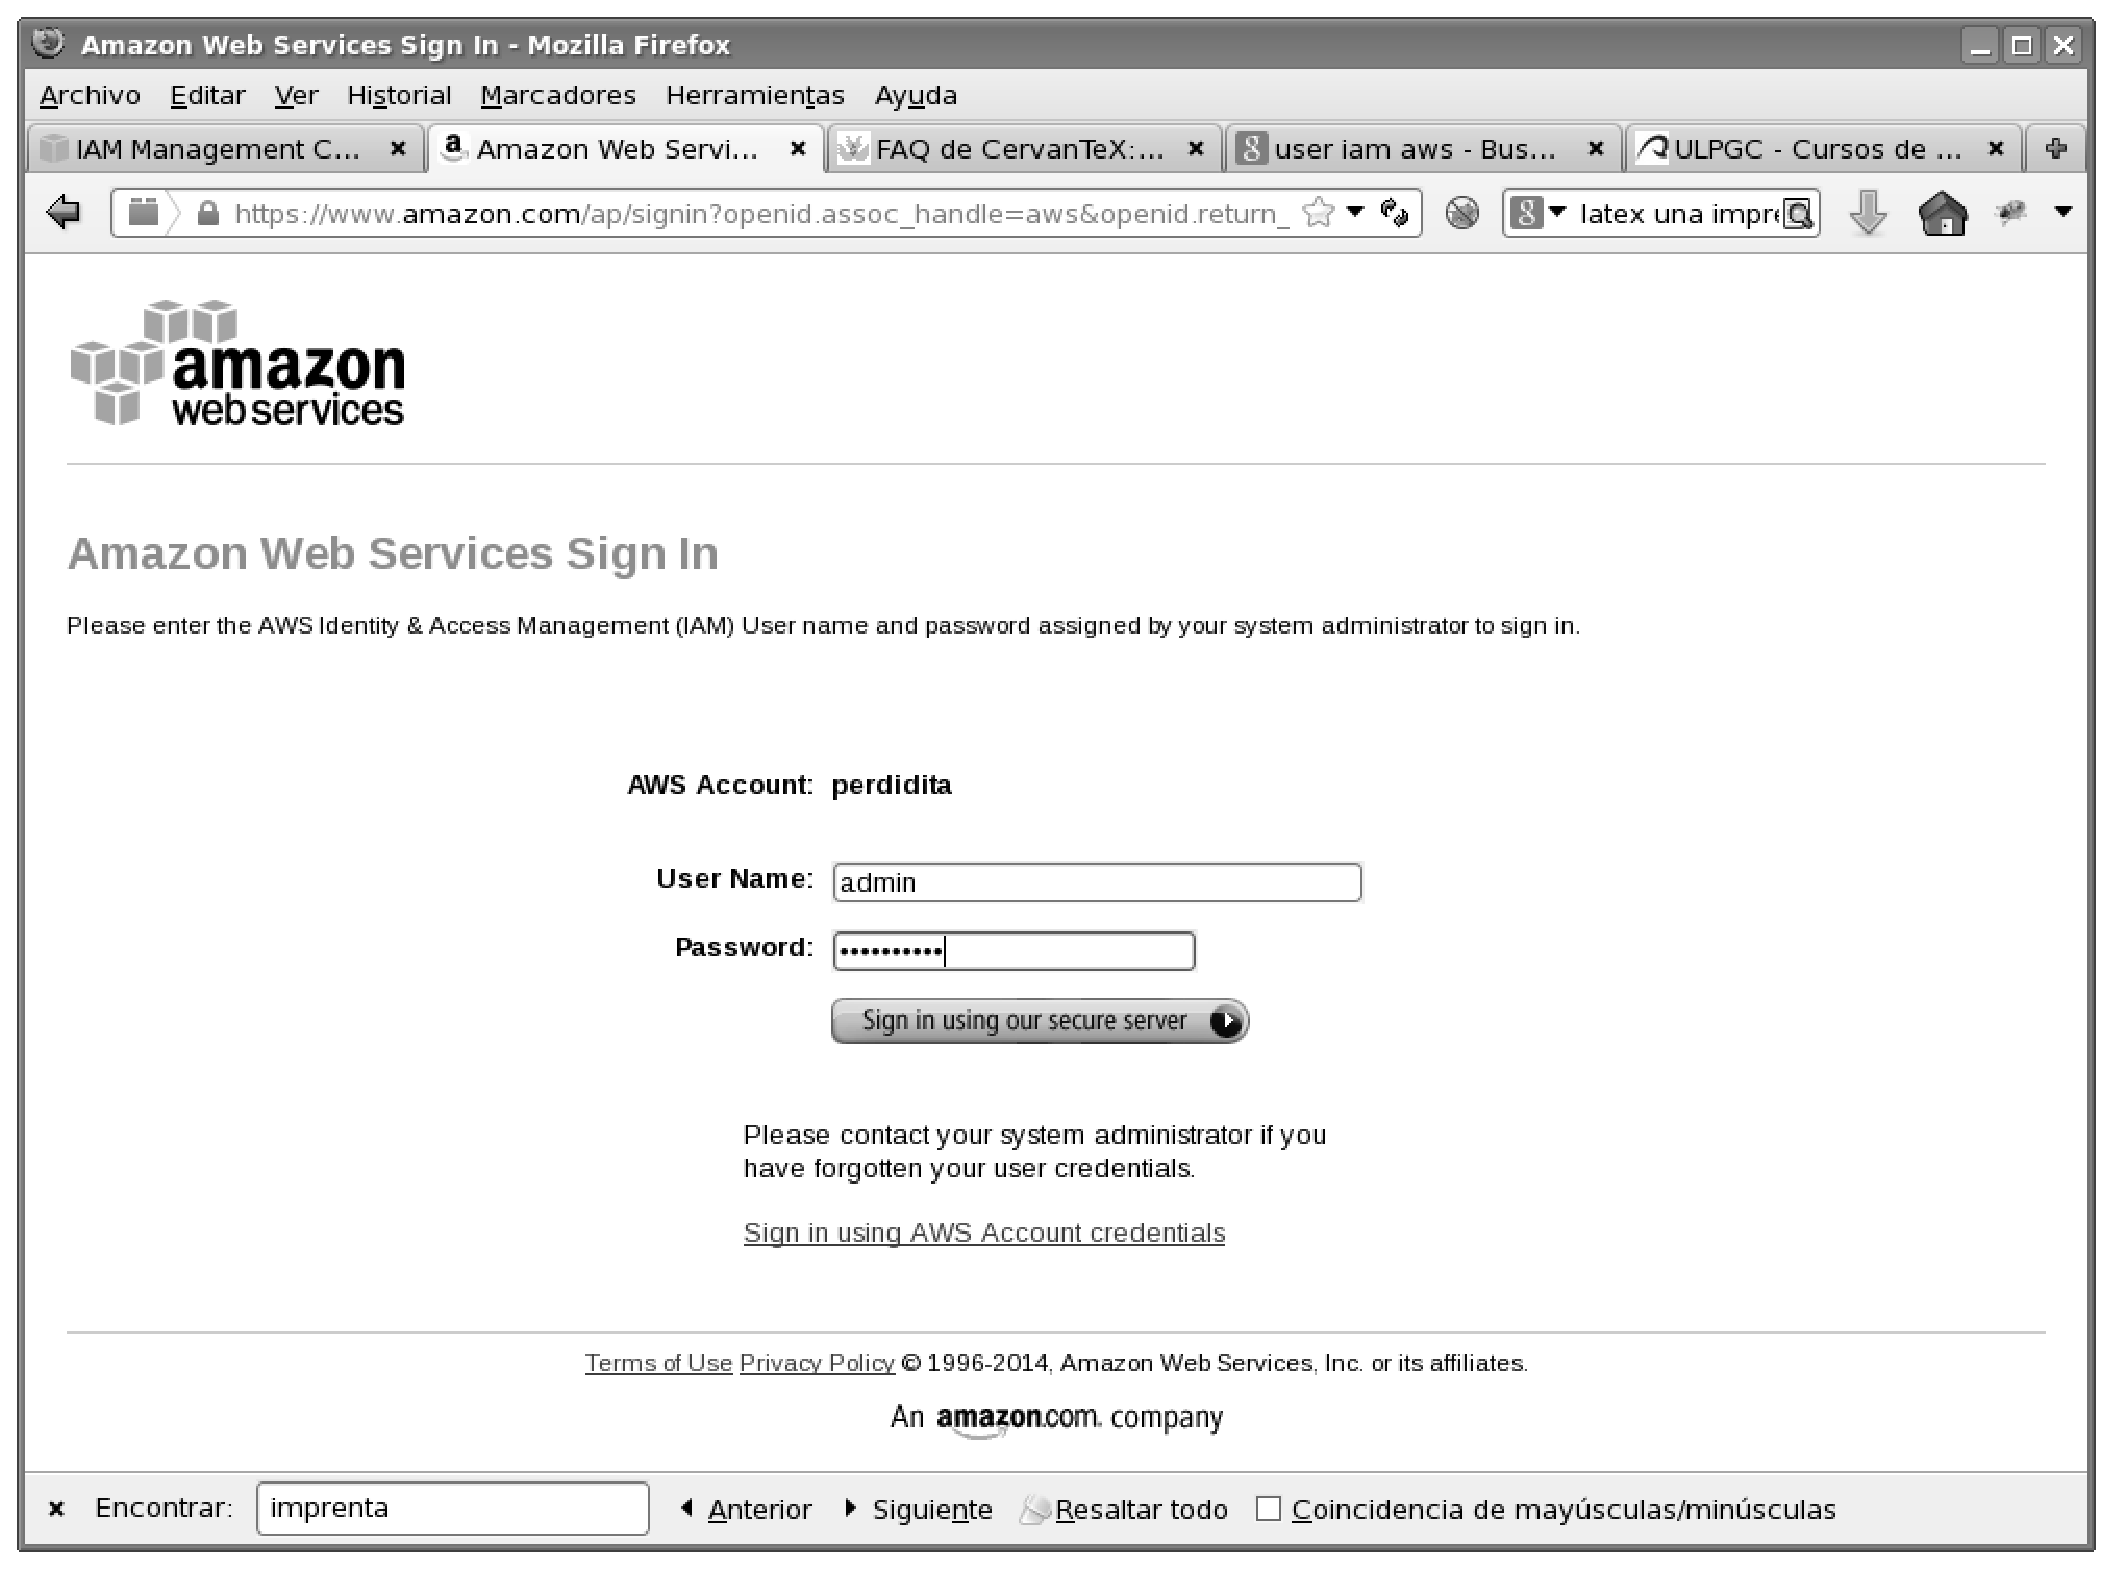
\includegraphics[scale=0.10]{siginurl1.eps}
\end{center}
\end{columns}
\end{itemize}
\end{frame}

%%%%%%%%%%%%%%%%%%%%%%%%%%%%%%%%%%%%%%%%%%%%%%%%%%%%%%%%%%%%%%%%%%%%%%%%%%%%%%
\section{Homework}
%%%%%%%%%%%%%%%%%%%%%%%%%%%%%%%%%%%%%%%%%%%%%%%%%%%%%%%%%%%%%%%%%%%%%%%%%%%%%
\begin{frame}[fragile]
\frametitle{Homework}
\begin{itemize}
\item Create a Group \texttt{``Developers''} with permissions to sign-in and manage \acrshort{ec2} instances
\item Create a user \texttt{``jsmith''} and include him in the \texttt{``Developers''} Group
\item Create an \acrshort{iam} User Sing-In URL with an alias
\item Login in your \acrshort{aws} as \texttt{``jsmith''}
\end{itemize}
\end{frame}

%%%%%%%%%%%%%%%%%%%%%%%%%%%%%%%%%%%%%%%%%%%%%%%%%%%%%%%%%%%%%%%%%%%%%%%%%%%%%%

%%%%%%%%%%%%%%%%%%%%%%%%%%%%%%%%%%%%%%%%%%%%%%%%%%%%%%%%%%%%%%%%%%%%%%%%%%%%%%


\end{document}
